\documentclass[a4paper,10pt]{article}
%\documentclass[dutch]{IEEEtran}
%\documentclass[a4paper,10pt]{scrartcl}
\usepackage[dutch]{babel}
\usepackage[utf8]{inputenc}
\usepackage[official]{eurosym}
\usepackage{url}
\usepackage[nottoc, numbib]{tocbibind}
%\usepackage[style=ieee, backend=bibtex]{biblatex}

\title{Conceptueel schaalmodel van een autonome Marsrover}
\author{Floris Kint \and Selwin Konijn \and Evert Leeuws \and Urban Lemmens \and Jan-Uwe Lorent \and Michiel Vanschoonbeek \and Vincent Vliegen \and Ruben Verhulst}
\date{\today}

\pdfinfo{%
  /Title    (Conceptueel schaalmodel van een autonome Marsrover)
  /Author   (Team 208: Floris Kint, Selwin Konijn, Evert Leeuws, Urban Lemmens, Jan-Uwe Lorent, Michiel Vanschoonbeek, Vincent Vliegen, Ruben Verhulst)
  /Creator  ()
  /Producer ()
  /Subject  ()
  /Keywords ()
}

\begin{document}
\maketitle
\newpage
\tableofcontents
\newpage
 
\section{Inleiding}
Bij het verkennen van de ruimte en andere hemellichamen zijn er verschillende 
factoren die tot problemen kunnen leiden. De grote afstand is daar één van. Op 
een andere planeet zou een verkenningsrover hierdoor een vertraging van 
inkomende en uitgaande signalen ondervinden. Deze vertraging zou tot problemen 
kunnen leiden bij het besturen van de rover. Dit probleem kan opgelost worden 
door de rover voor een deel autonoom te maken. Deze kan dan zelf een veilige weg 
vinden en obstakels ontwijken.

De marsrover Curiosity is een voorbeeld van zo’n autonome rover. Deze bezit 17 
camera's waarmee hij zijn omgeving kan aftasten. Aan de hand van de verzamelde 
informatie kan de Curiosity een veilig pad over het marsoppervlak vinden. Dit 
spaart tijd uit voor de bestuurders van de rover op aarde.\cite{NASACuriosity, 
NASA2013-259} 

De specifieke opdracht bestaat uit het ontwerpen van een wagentje dat autonoom 
een vooraf onbekend parcours moet afleggen. Het parcours is maximaal 12 m lang, 
minimaal 40 cm breed en de afbakenende muren zijn 18 cm hoog. De af te leggen 
weg bestaat uit rechte hoeken en er zijn geen plaatsen waarin het wagentje vast 
kan komen te zitten (er zijn geen doodlopende zijwegen). Het wagentje moet het 
parcours zo snel mogelijk afleggen en bij het bereiken van de finish een visueel 
of auditief signaal geven. De totaalprijs van het ontwerp mag maximaal \euro 80 
bedragen.

Met behulp van een afstandssensor verzamelt de wagen informatie over de 
omgeving. De Arduino Uno-controller ontvangt de metingen. Daarna verwerkt deze  
de informatie en zendt dan weer aan de hand van computercode signalen uit naar 
de motoren en het stuurmechanisme zodat de wagen op de juiste baan blijft. Op 
deze manier kan de wagen autonoom een onbekend parcours afleggen, zoals 
de opdracht vereist.

In dit verslag zal in het eerste deel de definitieve conceptkeuze, met name het 
mechanische en elektronische ontwerp aan bod komen. Ook de materiaalkeuze voor 
de rover komt hier aan bod. De volgende sectie “Experimenten” bevat de 
ontwerpberekeningen en de uitgevoerde experimenten. Deze zijn ondersteund met 
informatie uit bijlages A en B. Daarna volgt een bespreking van de resultaten 
van de demonstratie. Als laatste wordt het behalen van de deadlines besproken.
Doorheen het verslag zullen er enkele belangrijke bevindingen aan bod komen. De 
theoretische optimale overbrengingsverhouding kan bijvoorbeeld niet behaald 
worden. De luchtweerstand is pas merkbaar bij hoge snelheden en kan dus 
verwaarloosd worden bij het rijden op het parcours.  

 
\section{Conceptkeuze en ontwerp}
De lijst met productvereisten hielp bij het vinden van het beste idee. Het ontwerp dat het best voldeed aan de vereisten, een vierwieler met een stuurmechanisme gelijkaardig aan dat van een auto, kreeg verdere uitwerking.
Hierna volgt een besluit over de combinatie van sensoren waarmee de wagen uitgerust is om de omgeving zo goed mogelijk te kunnen aftasten. Rekening houdend met de prijs bleek een afstandssensor, gemonteerd op een servomotor het meest voordelig. Verder is er een elektromotor om de wagen aan te drijven en een servomotor om het stuurmechanisme aan te drijven. 

Een preciezere beschrijving van het mechanisch en elektronisch gedeelte volgt in de volgende paragrafen.

\subsection{Materialen}
In het bouwen van de wagen zijn verschillende materialen en onderdelen gebruikt. De belangrijkste zijn hieronder terug te vinden.

De bodemplaat van de wagen is van MDF (hout) en uitgesneden met behulp van een lasercutter. Het sturingsmechanisme is gebouwd uit Lego Technics en de  wielen hebben een doorsnede van 60 mm. Voor de overbrenging zijn er zes tandwielen van 26 mm en twee kleinere tandwielen van 5,2 mm doorsneden.
Een MM28 motor zorgt ervoor dat de wagen kan rijden. 

De wagen verzamelt zijn informatie met behulp van een IR-afstandssensor en een Arduino Uno-controller verwerkt deze informatie dan. Twee servomotors bewegen het sturingsmechanisme en de IR-sensor. Het geheel is verbonden met behulp van kabels die op een Printed Circuit Board gesoldeerd zijn. Een battery pack levert stroom aan de elektrische componenten. 

De volledige materiaallijst is opgenomen in Bijlage~\ref{bijlage:materiaallijst}. 


 
\subsection{Mechanisch}
Het wagentje is een vierwieler. Een model van de wagen bevindt zich in Figuur~\ref{image:auto-resultaat}. Aan de voorkant is langs beide kanten een 
rechthoek uitgesneden. Deze uitsnijdingen zorgen ervoor dat de wielen genoeg 
plaats hebben om te kunnen draaien. Achteraan is een as waarop beide 
achterwielen gefixeerd zijn. 
Op de achteras is een elektromotor (MM28) aangesloten die zorgt voor de 
aandrijving van de wagen. De motor staat via een reeks van tandwielen in 
verbinding met de achteras. Deze tandwielen zorgen voor de nodige overbrenging 
naar de wielen. Deze overbrenging heeft een verhouding van 1 op 125, waarbij de 
achteras 125 keer trager draait dan de motor.  De wagen remt door het 
uitschakelen van de motor. De rolweerstand en de wrijving veroorzaakt door de 
overbrenging, is voldoende om de wagen op tijd te laten stoppen.
De voorwielen staan elk op een aparte as. De twee assen zijn verbonden met een 
stuurmechanisme waardoor de voorwielen altijd parallel staan ten opzichte van 
elkaar. De wielen kunnen wel schuin komen te staan ten opzichte van de 
middenlijn. Hierdoor kan de auto gemakkelijk bochten nemen. De assen bewegen 
onder impuls van een servomotor. Deze servomotor drijft het sturingsmechanisme 
aan waardoor de wielen een hoek van ten hoogste 45 graden kunnen maken ten 
opzichte van de middenlijn. De afstandssensor is bovenop het sturingsmechanisme 
aangebracht, helemaal vooraan de wagen.
\begin{figure}
 \centering
 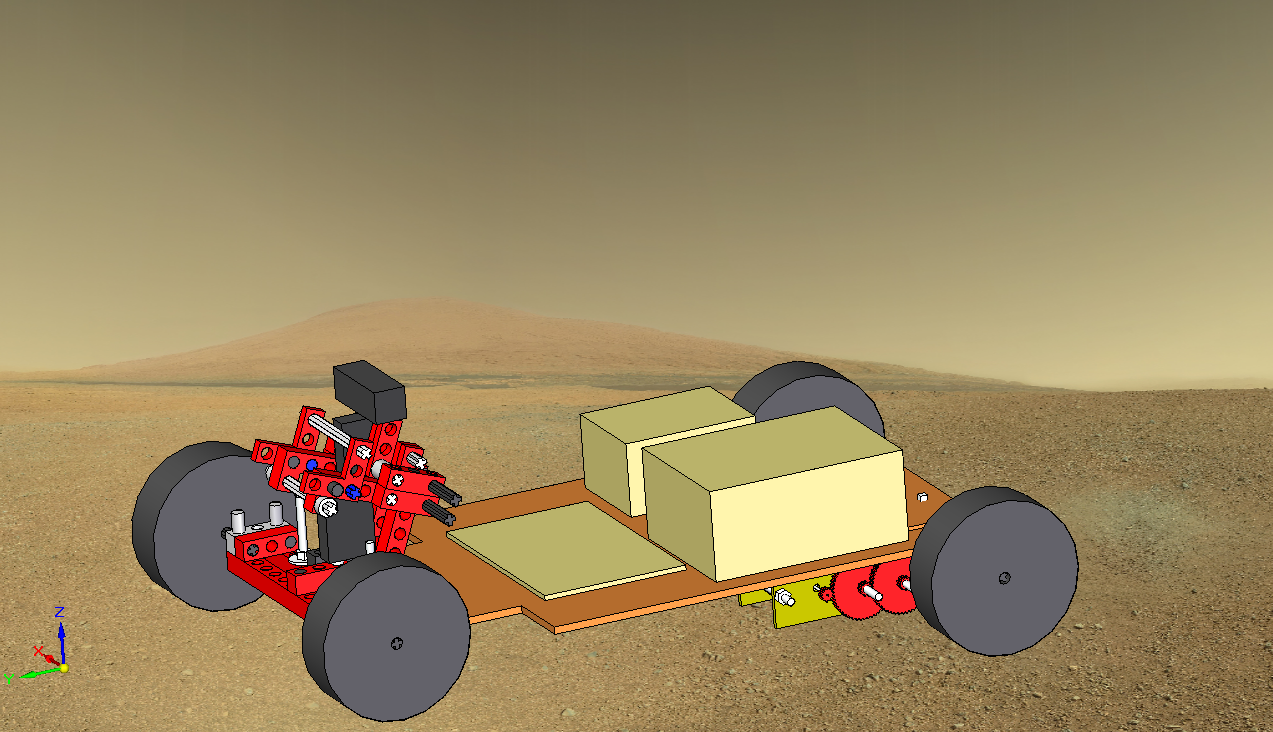
\includegraphics[width=\linewidth]{conceptkeuze-ontwerp/mechanisch/auto-resultaat.png}
 \caption{3D-model van het wagentje gemaakt met Solid Edge.}
 \label{image:auto-resultaat}
\end{figure}

De bodemplaat wordt schuin gemonteerd op beide assen en ligt hoger aan de 
achterkant. De plaat staat schuin omdat de motor en overbrenging aan de 
onderkant gemonteerd zijn. Hierdoor is er genoeg plaats over aan de bovenkant 
voor de elektronica en kunnen de tandwielen de draden niet beschadigen. 
Op de bovenkant van de bodemplaat komt de Arduino, de batterij en het Printed 
Circuit Board (PCB). Het gewicht wordt hierbij zo centraal mogelijk geplaatst, 
zodat het stuurmechanisme nog genoeg grip heeft om de koers van de wagen te 
wijzigen, zonder daarbij te veel weerstand te veroorzaken voor de servomotor. 
Bij een te hoge weerstand zou de servomotor de wielen niet op tijd kunnen 
draaien en zou de wagen de muur raken.

Het voordeel aan dit ontwerp is dat de stabiliteit, snelheid en wendbaarheid 
geoptimaliseerd worden. 

 
\subsection{Elektronisch}

 
\subsection{AI}
De aansturende software op de Arduinocontroler laat de radarsensor afwisselend links, vooruit en rechts de afstand meten. Afhankelijk van de gemeten waarden stuurt de software het wagentje bij.
Van zodra voor de afstandssensor vooruit een muur opmerkt, stopt het wagentje. Afhankelijk van de gemeten waarden links en rechts, weet de software aan welke kant het volgende deel van het traject zich bevindt.
Indien zich aan beide kanten een muur bevindt, is de rover op de bestemming aangekomen en knippert een LED.
Wanneer er voor het wagentje geen muur staat en de waarden links en rechts indiceren dat het wagentje zich tussen twee muren bevindt, maar dat de ene muur dichterbij is dan de andere, stuurt de software de baan van de wagen bij.

De software bestaat uit verschillende klassen die abstractie maken van de hardwarespecifieke commando's om de sensoren in te lezen en de actoren aan te sturen.
Zo is er een MyServo-, LedOutput-, Motor-, DistanceSensor-, MusicPlayer en PushButtonklasse. Deze laatste twee werden niet gebruikt in het uiteindelijke ontwerp, maar het programmeren van de skeletten gebeurde reeds in een eerste fase van het project.

De DrivingManagerklasse is de centrale unit van waaruit de wagen aangestuurd wordt. Deze klasse neemt de beslissingen zoals hierboven beschreven. 
DrivingManager kan de objecten manipuleren door middel van duidelijke commando's, zonder details over de onderliggende commando's. 
De methode setMotorSpeed in de klasse Motor regelt zo bijvoorbeeld de snelheid van de motoren en de staat van de relais, zodat ook achteruit gereden kan worden.

Om het testen van de aparte sensoren en actoren te vergemakkelijken, staan er ook enkele demo's in de DrivingManager-klasse. Deze zijn bedoeld om de specifieke elementen te testen. 
De methode radarDemo roteert bijvoorbeeld de servo waarop de afstandssensor gemonteerd is en de ingelezen waarden van de afstandssensor worden dan (geconverteerd naar centimeter) doorgestuurd via de Serial Monitor. Op die manier kan dit onderdeel gemakkelijker onderzocht worden op problemen als het aangesloten is aan de Arduino IDE\footnote{IDE: Integrated Development Environment (geïntegreerde ontwikkelomgeving).}.

De volledige code bevindt zich in Bijlage~\ref{bijlage:programma-code}.

 
\section{Experimenten}
\subsection{Rolweerstand}

Het kennen van de rolweerstand is belangrijk bij het berekenen van de snelheid van de wagen en voor het verlies van elektrische energie in warmtevorming.

De rolweerstand wordt berekend door de omzetting van potentiële energie naar kinetische energie te bestuderen. Met behulp van de wet van behoud van energie kan de verloren energie ten gevolge van de wrijving berekend worden aan de hand van het tweede postulaat van Newton.
Verdere uitleg en uitgebreide berekeningen staan in Bijlage~\ref{bijlage:rolweerstand}.

Uit experimenten blijkt dat de gebruikte wielen een wrijvingscoëfficiënt van 0.06 hebben.
\subsection{Luchtweerstand}


\subsection{Koppeloverdracht}


 
\subsection{Snelheidsmeting}
\subsection{Animatiefilmpje}

Een lineaire vergelijking bleek een erg goede benadering voor de bewegingsvergelijking van het wagentje (zie Bijlage~\ref{bijlage:animatiefilmpje}).
Het animatiefilmpje simuleert de beweging van het karretje dan ook alsof het een constante snelheid heeft gedurende het volledige parcours.

De Maplefile bevindt zich in Bijlage~\ref{bijlage:animatiefilmpje}. Met behulp van de voorgedefinieerde \verb|plot3d|-functies (\verb|polygonplot3d|), plot Maple het parcours en het wagentje in een opeenvolging van frames.
Verschillende zelfgedefinieerde procedures structureren het plotten van een frame door het onder te verdelen in enkele deeltaken. Zo zijn er de procedures \verb|plot_wagentje| en \verb|plot_wall_part| die voor een gegeven positie (en rotatie voor het wagentje), de nodige matrixbewerkingen uitvoeren en vervolgens het gevraagde object plotten.
Het parcours is gedefinieerd als een opeenvolging van punten. De muren en het wagentje worden opengetrokken op basis van hun coordinaten in het vlak. De bovenkant van de muren en het karretje zijn loodrechte translaties van het grondvlak. Telkens worden de overeenkomstige zijden als rechthoek geplot, zodat het model gesloten is.
De respectievelijke middens tussen de achterwielen en de voorwielen bevinden zich altijd op de lijn van het parcours. Met behulp van eenvoudige goniometrie wordt het karretje gedurende het rijden geroteerd zodat altijd aan deze voorwaarde voldaan is en de constante snelheid over de lijn behouden blijft. Deze vorm van rotatie is slechts een model en komt niet overeen met de bochten die het werkelijke ontwerp maakt.
De werkelijke rover stuurt enkel met de voorwielen en kan niet in rechte hoeken draaien, wat in het animatiefilmpje wel gebeurt.


\section{Resultaten demonstratie}
De marswagen is in mate van het mogelijke in orde gebracht voor de demonstratie. 
De servomotor van het radarsysteem, die tijdens enkele tests het begaf, is 
vervangen door een andere servomotor. De software echter is echter niet binnen 
de overige beschikbare tijd aangepast kunnen worden. Daarom wordt slechts een 
beperkt onderdeel van de gehele code geactiveerd. De marswagen zal hierdoor 
enkel in staat zijn rechtdoor te rijden en bij het tegenkomen van de muur zijn 
eindsignaal geven.
Naar aanvang van de demonstratie, wordt het wagentje geplaatst op het parcours. 
De wagen begint te rijden na het induwen van de reset knop. De wagen versnelt 
een korte tijd, waarna de motoren worden uitgeschakeld. Deze onderbreking dient 
als een snelheidsbeperking, dit geeft de tijd die nodig is voor het bijsturen 
van het wagentje. Echter bijsturen doet het niet, aangezien het draaien van de 
radar is uitgeschakeld. Zo komt het wagentje nog voor het einde van het eerste 
rechte stuk tot stilstand. Het wijkt lichtjes af waardoor de afstandsensor, die 
voorwaarts gericht staat, de linkerzijmuur waarneemt en het wagentje tot 
stilstand wordt gebracht. Ingesteld als eindsignaal, begint een van de LEDjes 
van de Arduino Uno-controller te branden. Dit wordt echter niet bemerkt door de 
assistenten en de jury, omdat dit maar een klein, onopvallend signaal is en er 
een GPIO kabel het zicht blokkeerde.
De marsauto heeft het parcours niet helemaal afgelegd zoals verwacht. De wagen 
haalde het einde van het eerste rechte stuk niet, dit door een lichte afwijking 
die niet kan worden gecorrigeerd. Wel geeft het een eindsignaal bij het bemerken 
van een muur op bepaalde afstand aan de voorzijde van het wagentje. Ook de 
snelheid die het wagentje maximaal bereikt, is laag genoeg om manoeuvres uit te 
voeren.
\section{Teamefficiëntie en deadlines}


 
\section{Discussie}
 
\section{Besluit}
test 2

\section{Bijlagen}
\subsection{Bijlage 1: Lijst van gebruikte symbolen}
$m$ = massa\\
$g$ = valversnelling\\
$G$ = universele gravitatieconstante ($6.6754*10^{-11} \frac{m^3}{s^2*kg}$)\\
$v$ = snelheid\\
$x$ = verplaatsing\\
$a$ = versnelling\\
$\mu$ = rolweerstandsco\"effici\"ent\\ 
$Cd$ = luchtweerstandsco\"effici\"ent\\
$F_{motor}$ = voortdrijvende kracht door motor\\
$F_{rol}$ = rolweerstand\\
$F_{lucht}$ = luchtweerstand\\
$\theta$ = hoek\\
$A$ = oppervlakte\\
$\rho$ = dichtheid\\
$\eta$ = overbrenging\\
$\omega$ = hoeksnelheid\\
$R$ = straal\\
$T$ = koppel van motor\\

\subsection{Bijlage 2: Berekening rolweerstand}

\subsubsection{De rolweerstand op Aarde}

Een belangrijke eigenschap van de Rover is de rolweerstand. Dit heeft een grote invloed in de effici\"entie van het rijden. Met een grote rolweerstand komt de wagen veel sneller tot stilstand dan bij een kleine rolweerstand. Het bepalen van de rolweerstand is niet moeilijk. Met behulp van een schuine plank is het mogelijk het verband te zoeken tussen de hoogte van waarop de wagen is losgelaten en de afstand die de wagen heeft afgelegd nadat het van de plank reed.\\
Wanneer de wagen boven op de plank staat, heeft het door de zwaartekracht een zekere potenti\"ele energie.
\begin{equation}
E_{pot}=m*g*h
\end{equation}
Wanneer de wagen naar beneden rolt, zet het die potenti\"ele energie om in kenetische energie.
\begin{equation}
E_{kin}=\frac{m*v^2}{2}
\end{equation}
Aan de onderkant van de helling is alles omgezet in kinetische energie. De snelheid $v$ is nu te berekenen door de vorige 2 formules aan elkaar gelijk te stellen. Voor het berekenen van deze snelheid wordt de wrijving met de grond tijdens het rijden op de helling verwaarloosd. Dit is echter een redelijke veronderstelling doordat de wrijving zeer klein is ten opzichte van de zwaartekracht.\\
Terwijl de wagen verder rolt, verliest het deze energie door de wrijving met de grond. Uit de bewegingsvergelijking hieronder kan de versnelling $a$ berekend worden.
\footnote{Deze vergelijking werd afgeleid door team 208 in P\&O opdracht 3}
\begin{equation}
x=\frac{1}{2}*\left(\frac{-v}{a}\right)^2+v*\left(\frac{-v}{a}\right)
\end{equation}
Terwijl de wagen verder rolt, spelen er drie krachten op in. Dit zijn de zwaartekracht, de normaalkracht en de wrijvingskracht. Aangezien de wagen horizontaal rijdt, heeft alleen de wrijvingskracht invloed op de versnelling. Met behulp van het $2\textsuperscript{de}$ Postulaat van Newton kan de rolweerstand bepaald worden.
\begin{equation}
F_{rol}=F_{res}=m*a
\end{equation}
Ten slotte wordt de wrijvingsco\"effici\"ent $\mu$ bepaald met behulp van de definitie van de rolweerstand.
\begin{equation}
\mu=\frac{F_{rol}}{F_{normaal}}=\frac{F_{rol}}{m*g}
\end{equation}
%Dit moet aangepast worden
%geen "worden" en verleden tijd
Om de onnauwkeurigheid van meetresultaten zo goed mogelijk te beperken, werd dit experiment zes keren herhaald. De definitieve wrijvingscoëffici\"ent is het gemiddelde van de zes bekomen coëfficiënten. deze waarde bedraagt:$$\mu=0.067$$
\pagebreak
\subsubsection{De rolweerstand op Mars}
Het vinden van de rolweerstand op Mars gebeurt op een zeer gelijkaardige manier als het vinden van de rolweerstand op Aarde. Het enige verschil is de gravitatieconstante $g$. Om de gravitatieconstante van Mars te berekenen, bestaat de volgende formule.
\begin{equation}
g=\frac{G*m_{Mars}}{\left(r_{Mars}\right)^2}
\end{equation}
Wanneer deze nieuwe gravitatieconstante ingevuld wordt in de vorige vergelijkingen, wordt de nieuwe rolweerstand $$F_{rol}=0.12N$$
\subsection{Bijlage 3: Berekening luchtweerstand}

Een ander belangrijke eigenschap van de rover is de luchtweerstand. Deze heeft maar weinig invloed bij lage snelheden, maar begint zeker mee te tellen zodra de snelheid stijgt. Het bepalen van de luchtweerstand gebeurt in twee stappen.\\
Eerst wordt met behulp van een krachtenevenwicht een differentiaalvergelijking opgesteld en opgelost. Hiermee wordt de theoretische baan van de wagen berekend. Dit staat wel nog altijd in functie van een onbekende $Cd$, de luchtweerstandsco\"effici\"ent.\\
Vervolgens wordt met behulp van video-analyse de feitelijke baan opgemeten. De werkelijke baan en de theoretische baan worden met alkaar vergeleken. Ten slotte wordt er een kleinste-kwadratische oplossing gezocht in voor $Cd$.\\
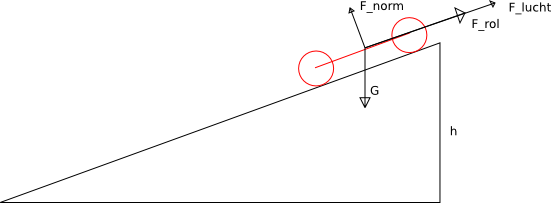
\includegraphics[width=10cm]{bijlagen/bijlage-3/luchtweerstand.png}
\subsubsection{Theoretische baan}
%Maple file theoretische baan
Wanneer de rover naar beneden rolt, werken er vier krachten op in, namelijk de zwaartekracht, de normaalkracht, de rolweerstand en de luchtweerstand. Voor het opstellen van de bewegingsvergelijking wordt de x-as evenwijdig met de helling gelegd. Zo is de versnelling alleen maar in de x-richting en moeten alleen maar de x-componenten van de krachten beschouwd worden.
\begin{equation} \label{eq:rolweerstand}
F_{rol}=-\mu*m*g*cos(\theta)
\end{equation}
\begin{equation} \label{eq:luchtweerstand}
F_{lucht}=-\frac{1}{2}*\rho_{lucht}*A*Cd*\left(\frac{dx}{dt}\right)^2
\end{equation}
\begin{equation} \label{eq:zwaartekracht}
F_{zwaartekracht}=m*g*sin(\theta)
\end{equation}
De bewegingsvergelijking wordt dus
\begin{equation}
F_{zwaartekracht} - F{rol}-F_{lucht}=m*\left(\frac{d^2x}{dt^2}\right)^2
\end{equation}
Deze vergelijking kan opgelost worden in functie van $Cd$.
\subsubsection{Feitelijke baan}
%Excel file praktische baan

\subsection{Bijlage 4: Berekening ideale overbrenging}

Wanneer de rover in beweging is, werken er in totaal drie krachten op in. Deze krachten zijn de voortdrijvende kracht door de motor, de wrijvingskracht door de rolweerstand en de wrijvingskracht door de luchtweerstand. De bewegingsvergelijking is dus:
\begin{equation} \label{eq:diff_vgl}
F_{motor}-F_{rol}-F_{lucht} = m*a
\end{equation}
De wrijvingskracht door de rolweerstand wordt bepaald met behulp van de volgende vergelijking.
\begin{equation} \label{eq:rolweerstand}
F_{rol}=\mu*m*g
\end{equation}
De wrijvingskracht door de luchtweerstand wordt bepaald met behulp van deze vergelijking.
%Hierin stelt A de oppervlakte voor die weerstand ondervindt door de lucht. De dichtheid van de lucht wordt voorgesteld door lucht en de snelheid van de rover door v.
\begin{equation} \label{eq:luchtweerstand}
F_{lucht}=\frac{1}{2} * \rho_{lucht} * Cd * A * v^2
\end{equation}
De aandrijvende kracht van de motor wordt verkregen met behulp van de volgende formule.
\begin{equation} \label{eq:motor}
F_{motor}=\frac{\eta}{R_{wiel}} * \frac{T_{max}-\left(T_{max}*\frac{dx}{dt}\right)}{\omega_{max}*R_{wiel}}
\end{equation}
Door vergelijkingen ~\ref{eq:rolweerstand},~\ref{eq:luchtweerstand} en ~\ref{eq:motor} in te vullen in vergelijking ~\ref{eq:diff_vgl} kan de vergelijking volledig opgelost worden. Als beginvoorwaarden wordt de snelheid en de plaats van de wagen op tijdstip 0 gelijk gesteld aan 0. De oplossing van de vergelijking is een vergelijking met de tijd in functie van de onbekende $\eta$. Deze wordt geoptimaliseerd voor een minimale tijd om $2.5$ meter af te leggen.\\
De optimale overbrengingsverhouding blijkt na numeriek in te vullen gelijk te zijn aan $\frac{1}{18}$
\subsection{Bijlage 5: Technische tekening}


\subsection{Bijlage 6: Programmacode}


\subsection{Bijlage 7: Financiën}


\subsection{Bijlage 8: Ganttchart}


\subsection{Bijlage 9: Animatiefilmpje}


\subsection{Bijlage 10: Poster}




\bibliographystyle{IEEEtran}
\bibliography{referenties}{}

\end{document}
